\section{I Reflective wrap }


In order to maximize the internal reflection to get better time resolution, choosing the right wrapping material became important, so the following study was done for this purpose.
One BC404 $6 \times 6 \times 120${cm}$^3 $ scintillator is wrapped using one layer of aluminized Mylar and several layers of Tedlar. Another same size scintillator is wrapped using one layer of the white paper material and the same amount of Tedlar. Hamamatsu PMTs serial FA0413 and FA0389 are mounted to the left and right ends, respectively, of the scintillator with the VM2000 wrapping and aluminized Mylar wrapping material. The detector is then placed as the middle bar in the 3 bar setup and voltages are set so as to bring the point of inflection on the ADC histograms to around 1000. Thresholds are set to 75mV. Data is collected until 180000-200000 events are recorded.

By comparing the time resolution of a scintillator bar wrapped in the VM2000 material with it in aluminized Mylar material, Fig.~\ref{f:wrap} shows that the VM2000 material does not yield significantly better time resolutions than the aluminized Mylar material. It was also noted that the setup with the white paper wrapping required greater voltage to achieve points of inflection around 1000 on the ADC histograms. Finally, we decide to use the cheaper aluminized Mylar as the wrapping material.
\vspace{20mm}
\begin{figure}[h]
\centerline{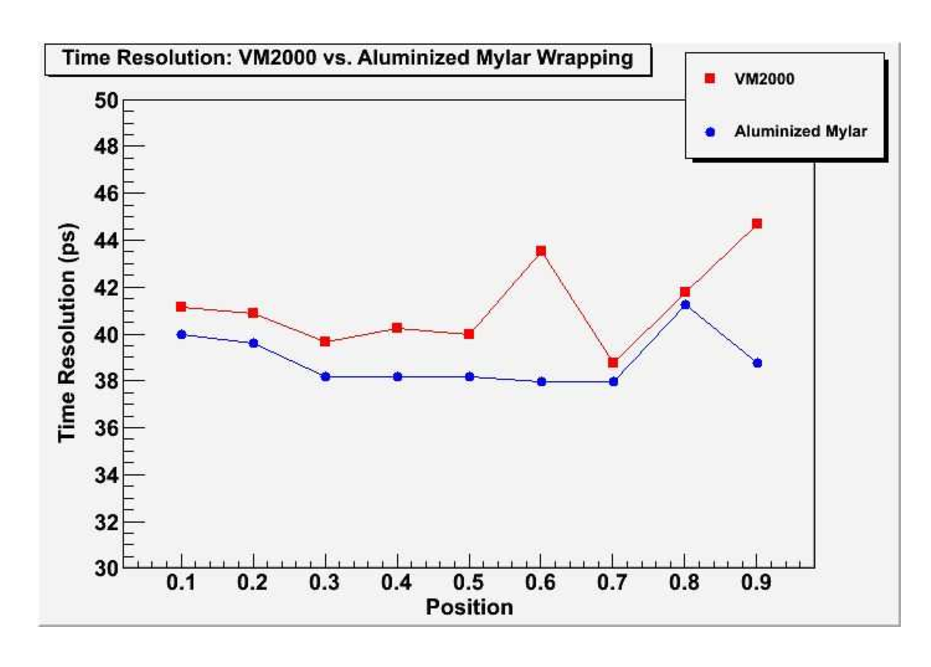
\includegraphics[width=13cm,height=10cm]{ye/fig_ye_wrap/R1.pdf}}
\caption{Wrap material}
\label{f:wrap}
\end{figure}

